\documentclass[11pt]{article}
\usepackage[a4paper,margin=1in]{geometry}
\usepackage{amsmath,amssymb,amsthm}
\usepackage{tikz}
\usetikzlibrary{arrows.meta,positioning}
\usepackage{xcolor}
\usepackage{booktabs}
\usepackage[hidelinks]{hyperref}
\hypersetup{pdftitle={Counting cycles in a Sylow 2-subgroup},pdfauthor={Vamshi Jandhyala}}
\setlength{\parskip}{0.4em}
\setlength{\parindent}{0pt}

\newtheorem{theorem}{Theorem}
\newtheorem{lemma}{Lemma}
\newtheorem{corollary}{Corollary}
\theoremstyle{remark}
\newtheorem*{remark}{Remark}
\newtheorem*{question}{Question}

\newcommand{\F}{\mathbb{F}}
\definecolor{swap}{RGB}{200,30,30}
\definecolor{minus}{RGB}{0,70,200}
\definecolor{plus}{RGB}{200,100,0}

\title{Counting cycles in a Sylow 2-subgroup}
\author{Vamshi Jandhyala}
\date{}

\begin{document}
\maketitle
\vspace{-2em}

\begin{abstract}
Let $P_n(q)$ count the permutations in a Sylow $2$-subgroup of $S_{2^n}$ by their number of cycles. Richard Stanley observed on MathOverflow that a closely related polynomial, shifted by a power of $2$, splits into two factors of equal degree, apparently irreducible. We note that the recurrence printed with the observation is off by one index from the Sylow polynomials, and prove that both families behave as observed: after the shift each is a product of two irreducible polynomials, for every $n$. Both reduce to iterating the triangular-number map $x\mapsto x(x+1)/2$. The factorization is a difference of two squares, and irreducibility follows by reducing modulo $5$, where the critical orbit of that map is $3\to1\to1$ and both factors take non-square values along it. All the algebra is formally verified in Lean.
\end{abstract}

\section{Symmetries of a tree}

Take a complete binary tree with $2^n$ leaves, and at each of its $2^n-1$ internal vertices decide whether to swap the two subtrees hanging below it (Figure~\ref{fig:tree}). Each choice of swaps permutes the leaves, and the $2^{2^n-1}$ permutations obtained form a group $G_{2^n}$. It is a Sylow $2$-subgroup of the symmetric group $S_{2^n}$, since $2^{2^n-1}$ is the largest power of $2$ dividing $(2^n)!$. Count its permutations by their number $\kappa(w)$ of cycles:
\[
P_n(q)=\sum_{w\in G_{2^n}}q^{\kappa(w)}.
\]
For $n=1$ the group is $S_2$, so $P_1=q^2+q$. For $n=2$ it is the symmetry group of a square, acting on the four corners: the identity has four cycles, the two reflections through a pair of corners have three, the half-turn and the two other reflections have two, and the two quarter-turns have one. So
\[
P_2(q)=q^4+2q^3+3q^2+2q .
\]
Now add the order of the group, $8$, and try to factor the result before reading on. It splits:
\[
P_2(q)+8=(q^2-q+2)(q^2+3q+4).
\]
The same happens one level up: $P_3+128$ is a product of two quartics, $P_4+2^{15}$ of two octics, and so on. Neither factor breaks further in these examples.

\begin{figure}[h]
\centering
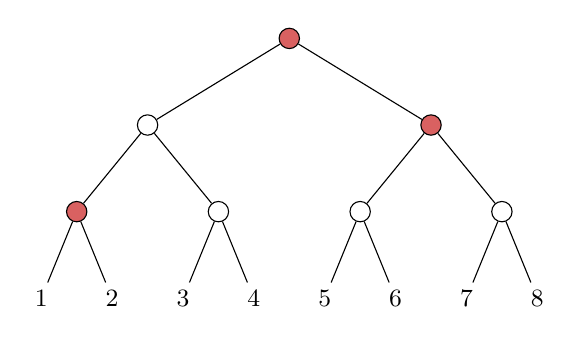
\begin{tikzpicture}[level distance=11mm, every node/.style={circle,draw,inner sep=2.6pt,fill=white},
  level 1/.style={sibling distance=36mm}, level 2/.style={sibling distance=18mm},
  level 3/.style={sibling distance=9mm}]
\node[fill=swap!70] {}
  child {node {}
    child {node[fill=swap!70] {} child {node[rectangle,draw=none] {\small 1}} child {node[rectangle,draw=none] {\small 2}}}
    child {node {} child {node[rectangle,draw=none] {\small 3}} child {node[rectangle,draw=none] {\small 4}}}}
  child {node[fill=swap!70] {}
    child {node {} child {node[rectangle,draw=none] {\small 5}} child {node[rectangle,draw=none] {\small 6}}}
    child {node {} child {node[rectangle,draw=none] {\small 7}} child {node[rectangle,draw=none] {\small 8}}}};
\end{tikzpicture}
\caption{An element of $G_8$: each shaded vertex swaps the two subtrees below it, and together the swaps permute the leaves $1,\dots,8$. There are $2^7=128$ ways to choose the shaded vertices, one for each element.}
\label{fig:tree}
\end{figure}

This was asked by Stanley on MathOverflow~\cite{MO}, in a slightly different form that we come back to in Section~\ref{sec:printed}. Darij Grinberg and Max Alekseyev found the factorization there~\cite{Grinberg,Alekseyev}; irreducibility of the factors was left open. We prove it.

\begin{theorem}\label{thm:main}
For every $n\ge2$,
\[
P_n(q)+|G_{2^n}|=A_n(q)\,B_n(q),
\]
where $A_n,B_n$ are monic integer polynomials of degree $2^{n-1}$, irreducible over $\mathbb Q$, and with equal coefficients in every degree above $2^{n-2}$.
\end{theorem}

\section{The recurrence, and an index slip}

Cutting the tree at its root shows how $P_{n+1}$ comes from $P_n$. An element of $G_{2^{n+1}}$ is a pair $(g_1,g_2)$ of elements of $G_{2^n}$, acting on the two halves, followed either by nothing or by the root swap~$\tau$. Without the swap, the cycles are those of $g_1$ together with those of $g_2$, so these elements contribute $P_n(q)^2$. With the swap, a point of the left half goes to the right half and comes back, so each cycle of $(g_1,g_2)\tau$ visits both halves, and its trace on the left half is a cycle of the product $g_2g_1$. As $(g_1,g_2)$ runs over all pairs, $g_2g_1$ runs over $G_{2^n}$ exactly $|G_{2^n}|$ times. Hence
\begin{equation}\label{eq:rec}
P_{n+1}=P_n\bigl(P_n+c_n\bigr),\qquad c_n=|G_{2^n}|=2^{2^n-1},\qquad P_0=q .
\end{equation}
This is the classical cycle index of a wreath product~\cite{Polya}, specialized to counting cycles. Setting $q=1$ gives $P_{n+1}(1)=c_n(2c_n)=c_{n+1}$, as it should.

Stanley's question~\cite{MO} defines instead $f_1=q^2+q$ and $f_{n+1}=f_n\bigl(f_n+2^{2^{n-1}-1}\bigr)$, and observes that $f_n+2^{2^{n-1}-1}$ factors for $n\ge3$. The constant $2^{2^{n-1}-1}$ is $c_{n-1}$, one index behind the order of the group being added in~\eqref{eq:rec}. The two families agree at $n=1$ and part ways at once: $f_2=q^4+2q^3+2q^2+q$ has $f_2(1)=6$, while $G_4$ has $8$ elements. Stanley's addendum, for odd primes, has the index right. Both families factor, for the same reason, and we treat both.

\section{Triangular numbers in disguise}

The recurrence~\eqref{eq:rec} has a cleaner form after scaling. Let
\[
T(x)=\frac{x(x+1)}2,
\]
the map sending $x$ to the $x$-th triangular number. Since $c_{n+1}=2c_n^2$, dividing~\eqref{eq:rec} by $c_{n+1}$ gives $P_{n+1}/c_{n+1}=T(P_n/c_n)$. With $P_0=q$ and $c_0=1$, this says
\[
P_n(q)=c_n\,T^{n}(q),
\]
where $T^n$ is the $n$-fold iterate. So counting cycles in the tree's symmetries is the same as applying the triangular-number map $n$ times, up to the scalar $c_n$. Since $T(1)=1$, this gives $P_n(1)=c_n$ again. In the same way the printed family is $f_n=c_{n-1}\,T^{n-1}(q^2+q)$: it iterates the same map from a different starting polynomial.

\section{Why it factors}

Adding $c_n$ to $P_n$ adds $1$ to $T^n(q)$, so the question is why $T^n(q)+1$ factors. Two steps of $T$ suffice. Write $y=T(z)$ and $w=z^2+z=2y$. Then
\[
T(y)+1=\frac{y^2+y+2}{2}=\frac{w^2+2w+8}{8}=\frac{(w+3)^2-(4w+1)}{8}.
\]
The point is that $4w+1=4z^2+4z+1=(2z+1)^2$ is itself a square. So the numerator is a difference of two squares:
\begin{equation}\label{eq:two}
T(T(z))+1=\frac{(w+3-2z-1)(w+3+2z+1)}{8}=\frac{h_-(z)\,h_+(z)}{8},
\end{equation}
where $h_-(z)=z^2-z+2$ and $h_+(z)=z^2+3z+4$.
Substituting $z=T^{n-2}(q)$ factors $T^n(q)+1$ for every $n\ge2$. Clearing denominators, with $c_n=8c_{n-2}^4$,
\[
P_n+c_n=A_nB_n,\qquad A_n=c_{n-2}^2\,h_-\bigl(T^{n-2}(q)\bigr),\quad B_n=c_{n-2}^2\,h_+\bigl(T^{n-2}(q)\bigr).
\]
In terms of the recurrence itself, using $c_{n-2}^2T^{n-2}(q)^2=P_{n-1}-c_{n-2}P_{n-2}$,
\[
A_n=P_{n-1}-2c_{n-2}P_{n-2}+c_{n-1},\qquad B_n=P_{n-1}+2c_{n-2}P_{n-2}+2c_{n-1},
\]
which are monic with integer coefficients and of degree $2^{n-1}$. This is the shape of Grinberg's factorization of the printed family~\cite{Grinberg}. Their difference $4c_{n-2}P_{n-2}+c_{n-1}$ has degree only $2^{n-2}$, so $A_n$ and $B_n$ agree in every coefficient above that degree: the agreement Stanley noticed.

\section{Why the halves do not factor}

A monic integer polynomial that is irreducible modulo a prime is irreducible over $\mathbb Q$, since any factorization over $\mathbb Q$ can be taken to be over $\mathbb Z$ with monic factors (Gauss's lemma) and would survive reduction. We reduce modulo $5$. The scalars $c_k$ are powers of $2$, which are units modulo $5$, so it is enough to show that $h_\pm\circ T^{k}$ is irreducible over $\F_5$ for every $k\ge0$.

Over $\F_5$ the nonzero squares are $1$ and $4$, and the non-squares are $2$ and $3$. Both $h_-$ and $h_+$ have discriminant $-7\equiv3$, a non-square, so both are irreducible. To go from $h_\pm\circ T^{k}$ to $h_\pm\circ T^{k+1}$ we compose once more with the quadratic $T$, and one lemma controls that step.

\begin{lemma}\label{lem:comp}
Let $\F$ be a finite field of odd characteristic, $G\in\F[x]$ irreducible of even degree $d$ with square leading coefficient, and $V(x)=ax^2+bx+e$ with $a\ne0$ and critical value $v=V(-b/2a)$. If $G(v)$ is not a square in $\F$, then $G\circ V$ is irreducible, of even degree $2d$, with square leading coefficient.
\end{lemma}

\begin{proof}
Let $\alpha$ be a root of $G$ and $K=\F(\alpha)$, a field of degree $d$ over $\F$. Suppose for the moment that $V(x)-\alpha$ is irreducible over $K$, and let $\beta$ be one of its roots. Then $G(V(\beta))=G(\alpha)=0$, and $\alpha=V(\beta)$ lies in $\F(\beta)$, so $[\F(\beta):\F]=[K(\beta):K]\,[K:\F]=2d$. A root of $G\circ V$ of degree $2d$, the full degree of $G\circ V$, means that $G\circ V$ is irreducible. It remains to show that $V(x)-\alpha$ is irreducible over $K$. The quadratic $V(x)-\alpha$ is irreducible over $K$ exactly when its discriminant $\Delta=b^2-4a(e-\alpha)=4a(\alpha-v)$ is not a square in $K$. Take norms from $K$ to $\F$. The conjugates of $\alpha$ are the $d$ roots $\alpha_i$ of $G$, and if $c$ is the leading coefficient of $G$ then $\prod_i(v-\alpha_i)=G(v)/c$, so
\[
N_{K/\F}(\Delta)=(4a)^d\prod_i(\alpha_i-v)=(4a)^d\,\frac{G(v)}{c}\qquad(d\text{ even}).
\]
Here $(4a)^d$ and $c$ are squares, so $N(\Delta)$ is a non-square. The norm of a square is a square, so $\Delta$ is not a square in $K$. Finally the degree $2d$ is even and the leading coefficient $c\,a^d$ is a square.
\end{proof}

This is the quadratic case of Capelli's lemma, written so that it can be checked by hand; the same computation drives the study of irreducible iterates of quadratic polynomials~\cite{Jones,JonesBoston,GNOS}.

The critical point of $T(x)=x(x+1)/2$ is $-1/2$, and its critical value is $-1/8$, which is $3$ in $\F_5$. Iterating $T$ from there gives
\[
T(3)=6\equiv1,\qquad T(1)=1,
\]
so the critical orbit is $3\to1\to1\to\cdots$ (Figure~\ref{fig:orbit}). We need $h_\pm\circ T^{k}$ to be a non-square at $3$ for each $k$. For $k=0$ this is $h_-(3)=8\equiv3$ and $h_+(3)=22\equiv2$. For $k\ge1$ the value is $h_\pm(T^{k}(3))=h_\pm(1)$, which is $h_-(1)=2$ and $h_+(1)=8\equiv3$. All four are non-squares.

\begin{figure}[h]
\centering
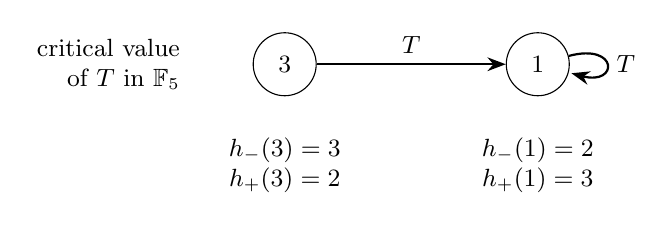
\begin{tikzpicture}[>=Stealth, node distance=24mm, every node/.style={font=\small}]
\node[circle,draw,minimum size=8mm] (c) {$3$};
\node[circle,draw,minimum size=8mm,right=of c] (o) {$1$};
\draw[->,thick] (c) -- node[above] {$T$} (o);
\draw[->,thick] (o) edge[loop right] node[right] {$T$} (o);
\node[below=4mm of c, align=center] {$h_-(3)=3$\\ $h_+(3)=2$};
\node[below=4mm of o, align=center] {$h_-(1)=2$\\ $h_+(1)=3$};
\node[left=8mm of c, align=right] {critical value\\ of $T$ in $\F_5$};
\end{tikzpicture}
\caption{The critical orbit of $T$ in $\F_5$, with the values of the two factors along it. All are non-squares, which is what Lemma~\ref{lem:comp} needs at every step.}
\label{fig:orbit}
\end{figure}

Now induct on $k$. The base $h_\pm$ is irreducible, monic, of degree $2$. If $H=h_\pm\circ T^{k}$ is irreducible of even degree with square leading coefficient, then $H(3)$ is a non-square by the table above, and Lemma~\ref{lem:comp} with $V=T$ shows that $H\circ T=h_\pm\circ T^{k+1}$ has the same three properties. So every $h_\pm\circ T^{k}$ is irreducible over $\F_5$, and Theorem~\ref{thm:main} follows.

The leading coefficient of $T$ is $1/2\equiv3$, a non-square, so the hypothesis on the leading coefficient is not automatic. It survives each step because $d$ is even, so $3^d$ is a square.

\section{The polynomials as printed}\label{sec:printed}

For the printed family $f_n=c_{n-1}\,T^{n-1}(Q)$, with $Q(q)=q^2+q$, the same identity~\eqref{eq:two} with $z=T^{n-3}(Q)$ gives $f_n+c_{n-1}=\tilde A_n\tilde B_n$ for $n\ge3$, where $\tilde A_n=c_{n-3}^2\,h_-(T^{n-3}(Q))$ and $\tilde B_n=c_{n-3}^2\,h_+(T^{n-3}(Q))$ are Grinberg's factors~\cite{Grinberg}. For instance $f_3+8=(q^4+2q^3-q+2)(q^4+2q^3+4q^2+3q+4)$.

\begin{corollary}
For every $n\ge3$, the two factors of $f_n+2^{2^{n-1}-1}$ are irreducible over $\mathbb Q$, have degree $2^{n-1}$, and agree in every coefficient above degree $2^{n-2}$.
\end{corollary}

\begin{proof}
Modulo $5$ the factors are unit multiples of $H\circ Q$ with $H=h_\pm\circ T^{n-3}$, which is irreducible of even degree with square leading coefficient, as shown above. The critical value of $Q$ is $-1/4\equiv1$, and $H(1)=h_\pm(1)\in\{2,3\}$ is a non-square because $1$ is fixed by $T$. One more application of Lemma~\ref{lem:comp} finishes the proof. The coefficient agreement is the degree count of the previous section.
\end{proof}

The prime $5$ is not arbitrary. Modulo $3$, for example, the critical value of $Q$ is $2$, then $T(2)=0$, and $h_+(0)=4\equiv1$ is a square; indeed some of the factors split modulo $3$, and also modulo $7$.

\section{Odd primes}

Stanley's addendum~\cite{MO} asks the same question for a Sylow $p$-subgroup of $S_{p^n}$, with $f_{1,p}=q^p+(p-1)q$ and
\[
f_{n+1,p}=f_{n,p}\bigl(f_{n,p}^{\,p-1}+(p-1)p^{p^n-1}\bigr).
\]
The scaling of Section~3 works for every $p$. With $\Phi_p(x)=\bigl(x^p+(p-1)x\bigr)/p$, one finds $f_{n,p}=p^{e_n}\,\Phi_p^{\,n}(q)$ with $e_n=(p^n-1)/(p-1)$, and the polynomial whose factorization is asked about becomes
\[
f_{n,p}^{\,p-1}+(p-1)p^{p^n-1}=p^{p^n-1}\,H_p\bigl(\Phi_p^{\,n}(q)\bigr),\qquad H_p(x)=x^{p-1}+p-1 .
\]
For $p=2$ this is the $T^n(q)+1$ above. For $p=5$, $H_5(x)=x^4+4$ splits by Sophie Germain's identity, $x^4+4=(x^2-2x+2)(x^2+2x+2)$, which is the factorization Stanley points out. For $p=3$ and $p=7$ the polynomial $H_p(\Phi_p^{\,n})$ is irreducible for $n\le3$ and $n\le2$ respectively, and for $p=5$ both Sophie Germain factors stay irreducible for $n\le3$; we checked these by computer. The method above uses that $T$ has degree $2$, so a single critical value controls every step. For $p\ge3$ the map $\Phi_p$ has $p-1$ critical points, and we do not know a proof.

\begin{question}
Is $H_p\circ\Phi_p^{\,n}$ irreducible over $\mathbb Q$ for every odd prime $p\ne5$ and every $n$? For $p=5$, are both factors $(x^2\mp2x+2)\circ\Phi_5^{\,n}$ irreducible?
\end{question}

\section*{Verification}

Every algebraic statement above is formally verified in Lean~4 with Mathlib~\cite{mathlib}: Lemma~\ref{lem:comp} with the norm computation, the recurrence and its factorization for both families, the agreement of top coefficients, and irreducibility over $\F_5$, $\mathbb Z$ and $\mathbb Q$ for every $n$. The proofs use only the standard axioms. Two things are not formalized: the identification of $P_n$ with the cycle count of $G_{2^n}$, which is the classical recurrence~\eqref{eq:rec}, and the computer data for odd primes. A separate program, sharing no code with the formal proofs, checks the cycle counts of $G_{2^n}$ by listing the group for $n\le4$, the factorizations for $n\le8$, irreducibility modulo~$5$ up to degree~$128$, Lemma~\ref{lem:comp} on random examples, and the data for odd primes. The code is at \url{https://github.com/jvvk/mathematics}.

\section*{Acknowledgment}

The author used two AI assistants, Codex (OpenAI) and Claude Opus~5.5 (Anthropic). Codex found the reduction to the triangular-number map and the modulo-$5$ argument, and wrote the first formal proof. Claude noticed the index slip, extended the argument and the formal proof to the Sylow polynomials, wrote the independent checking program and drafted the text. The author directed the work, checked the results and is responsible for the contents.

\begin{thebibliography}{9}
\bibitem{Alekseyev} M. Alekseyev, answer to~\cite{MO}, \url{https://mathoverflow.net/a/489364}.
\bibitem{GNOS} D. G\'omez-P\'erez, A. P. Nicol\'as, A. Ostafe and D. Sadornil, Stable polynomials over finite fields, \emph{Rev. Mat. Iberoam.} \textbf{30} (2014), 523--535.
\bibitem{Grinberg} D. Grinberg, answer to~\cite{MO}, \url{https://mathoverflow.net/a/489336}.
\bibitem{Jones} R. Jones, The density of prime divisors in the arithmetic dynamics of quadratic polynomials, \emph{J. Lond. Math. Soc. (2)} \textbf{78} (2008), 523--544.
\bibitem{JonesBoston} R. Jones and N. Boston, Settled polynomials over finite fields, \emph{Proc. Amer. Math. Soc.} \textbf{140} (2012), 1849--1863.
\bibitem{mathlib} The mathlib Community, The Lean mathematical library, in \emph{Proceedings of the 9th ACM SIGPLAN International Conference on Certified Programs and Proofs} (2020), 367--381.
\bibitem{Polya} G. P\'olya and R. C. Read, \emph{Combinatorial Enumeration of Groups, Graphs, and Chemical Compounds}, Springer, New York, 1987.
\bibitem{MO} R. P. Stanley, Unexpected factorization of a polynomial defined recursively, MathOverflow question 489315, \url{https://mathoverflow.net/q/489315}.
\end{thebibliography}

\end{document}
